%%
%% Automatically generated file from DocOnce source
%% (https://github.com/hplgit/doconce/)
%%

% #define PREAMBLE

% #ifdef PREAMBLE
%-------------------- begin preamble ----------------------

\documentclass[%
oneside,                 % oneside: electronic viewing, twoside: printing
final,                   % draft: marks overfull hboxes, figures with paths
10pt,french]{article}

\listfiles               %  print all files needed to compile this document

\usepackage{relsize,makeidx,color,setspace,amsmath,amsfonts,amssymb}
\usepackage[table]{xcolor}
\usepackage{bm,ltablex,microtype}

\usepackage[pdftex]{graphicx}

% Packages for typesetting blocks of computer code
\usepackage{fancyvrb,framed,moreverb}

% Define colors
\definecolor{orange}{cmyk}{0,0.4,0.8,0.2}
\definecolor{tucorange}{rgb}{1.0,0.64,0}
\definecolor{darkorange}{rgb}{.71,0.21,0.01}
\definecolor{darkgreen}{rgb}{.12,.54,.11}
\definecolor{myteal}{rgb}{.26, .44, .56}
\definecolor{gray}{gray}{0.45}
\definecolor{mediumgray}{gray}{.8}
\definecolor{lightgray}{gray}{.95}
\definecolor{brown}{rgb}{0.54,0.27,0.07}
\definecolor{purple}{rgb}{0.5,0.0,0.5}
\definecolor{darkgray}{gray}{0.25}
\definecolor{darkblue}{rgb}{0,0.08,0.45}
\definecolor{darkblue2}{rgb}{0,0,0.8}
\definecolor{lightred}{rgb}{1.0,0.39,0.28}
\definecolor{lightgreen}{rgb}{0.48,0.99,0.0}
\definecolor{lightblue}{rgb}{0.53,0.81,0.92}
\definecolor{lightblue2}{rgb}{0.3,0.3,1.0}
\definecolor{lightpurple}{rgb}{0.87,0.63,0.87}
\definecolor{lightcyan}{rgb}{0.5,1.0,0.83}

\colorlet{comment_green}{green!50!black}
\colorlet{string_red}{red!60!black}
\colorlet{keyword_pink}{magenta!70!black}
\colorlet{indendifier_green}{green!70!white}

% Backgrounds for code
\definecolor{cbg_gray}{rgb}{.95, .95, .95}
\definecolor{bar_gray}{rgb}{.92, .92, .92}

\definecolor{cbg_yellowgray}{rgb}{.95, .95, .85}
\definecolor{bar_yellowgray}{rgb}{.95, .95, .65}

\colorlet{cbg_yellow2}{yellow!10}
\colorlet{bar_yellow2}{yellow!20}

\definecolor{cbg_yellow1}{rgb}{.98, .98, 0.8}
\definecolor{bar_yellow1}{rgb}{.98, .98, 0.4}

\definecolor{cbg_red1}{rgb}{1, 0.85, 0.85}
\definecolor{bar_red1}{rgb}{1, 0.75, 0.85}

\definecolor{cbg_blue1}{rgb}{0.87843, 0.95686, 1.0}
\definecolor{bar_blue1}{rgb}{0.7,     0.95686, 1}

%\setlength{\fboxsep}{-1.5mm}  % adjust cod_vpad/pro_vpad background box

%% Background for code blocks (parameter is color name)

%% pro/cod_vpad: gives some vertical padding before and after the text
%% (but has more simplistic code than _cod/pro_tight+cod/pro).
%% pro/cod_vpad can be used to enclose Verbatim or lst begin/end for code.
%% pro/cod calls _pro/cod_tight and has very little vertical padding,
%% used to enclose Verbatim and other begin/end for code.
%% (pro/cod is what the ptex2tex program could produce with the
%% Blue/BlueBar definitions in .ptex2tex.cfg.)

\newenvironment{cod_vpad}[1]{
   \def\FrameCommand{\colorbox{#1}}
   \MakeFramed{\FrameRestore}}
   {\endMakeFramed}

\newenvironment{_cod_tight}[1]{
   \def\FrameCommand{\colorbox{#1}}
   \FrameRule0.6pt\MakeFramed {\FrameRestore}\vskip3mm}
   {\vskip0mm\endMakeFramed}

\newenvironment{cod}[1]{
\bgroup\rmfamily
\fboxsep=0mm\relax
\begin{_cod_tight}{#1}
\list{}{\parsep=-2mm\parskip=0mm\topsep=0pt\leftmargin=2mm
\rightmargin=2\leftmargin\leftmargin=4pt\relax}
\item\relax}
{\endlist\end{_cod_tight}\egroup}

%% Background for complete program blocks (parameter 1 is color name
%% for background, parameter 2 is color for left bar)
\newenvironment{pro_vpad}[2]{
   \def\FrameCommand{\color{#2}\vrule width 1mm\normalcolor\colorbox{#1}}
   \MakeFramed{\FrameRestore}}
   {\endMakeFramed}

\newenvironment{_pro_tight}[2]{
   \def\FrameCommand{\color{#2}\vrule width 1mm\normalcolor\colorbox{#1}}
   \FrameRule0.6pt\MakeFramed {\advance\hsize-2mm\FrameRestore}\vskip3mm}
   {\vskip0mm\endMakeFramed}

\newenvironment{pro}[2]{
\bgroup\rmfamily
\fboxsep=0mm\relax
\begin{_pro_tight}{#1}{#2}
\list{}{\parsep=-2mm\parskip=0mm\topsep=0pt\leftmargin=2mm
\rightmargin=2\leftmargin\leftmargin=4pt\relax}
\item\relax}
{\endlist\end{_pro_tight}\egroup}

\usepackage{minted}
\usemintedstyle{default}

\usepackage[T1]{fontenc}
%\usepackage[latin1]{inputenc}
\usepackage{ucs}
\usepackage[utf8x]{inputenc}

\usepackage{lmodern}         % Latin Modern fonts derived from Computer Modern

% Hyperlinks in PDF:
\definecolor{linkcolor}{rgb}{0,0,0.4}
\usepackage{hyperref}
\hypersetup{
    breaklinks=true,
    colorlinks=true,
    linkcolor=linkcolor,
    urlcolor=linkcolor,
    citecolor=black,
    filecolor=black,
    %filecolor=blue,
    pdfmenubar=true,
    pdftoolbar=true,
    bookmarksdepth=3   % Uncomment (and tweak) for PDF bookmarks with more levels than the TOC
    }
%\hyperbaseurl{}   % hyperlinks are relative to this root

\setcounter{tocdepth}{2}  % levels in table of contents

% Tricks for having figures close to where they are defined:
% 1. define less restrictive rules for where to put figures
\setcounter{topnumber}{2}
\setcounter{bottomnumber}{2}
\setcounter{totalnumber}{4}
\renewcommand{\topfraction}{0.95}
\renewcommand{\bottomfraction}{0.95}
\renewcommand{\textfraction}{0}
\renewcommand{\floatpagefraction}{0.75}
% floatpagefraction must always be less than topfraction!
% 2. ensure all figures are flushed before next section
\usepackage[section]{placeins}
% 3. enable begin{figure}[H] (often leads to ugly pagebreaks)
%\usepackage{float}\restylefloat{figure}

% --- fancyhdr package for fancy headers ---
\usepackage{fancyhdr}
\fancyhf{} % sets both header and footer to nothing
\renewcommand{\headrulewidth}{0pt}
\fancyfoot[LE,RO]{\thepage}
% Ensure copyright on titlepage (article style) and chapter pages (book style)
\fancypagestyle{plain}{
  \fancyhf{}
  \fancyfoot[C]{{\footnotesize \copyright\ 2020, Ahmed Ammar. Released under CC Attribution 4.0 license}}
%  \renewcommand{\footrulewidth}{0mm}
  \renewcommand{\headrulewidth}{0mm}
}
% Ensure copyright on titlepages with \thispagestyle{empty}
\fancypagestyle{empty}{
  \fancyhf{}
  \fancyfoot[C]{{\footnotesize \copyright\ 2020, Ahmed Ammar. Released under CC Attribution 4.0 license}}
  \renewcommand{\footrulewidth}{0mm}
  \renewcommand{\headrulewidth}{0mm}
}

\pagestyle{fancy}


\usepackage{framed,wrapfig}

% --- begin definitions of admonition environments ---

% Admonition style "grayicon" has colored background, no frame, and an icon
% Admon "notice"
\definecolor{grayicon_notice_background}{rgb}{0.91,0.91,0.91}
% \fboxsep sets the space between the text and the box
\newenvironment{noticeshaded}
{\def\FrameCommand{\fboxsep=3mm\colorbox{grayicon_notice_background}}
 \MakeFramed {\advance\hsize-\width \FrameRestore}}{\endMakeFramed}

\newenvironment{notice_grayiconadmon}[1][À noter]{
\begin{noticeshaded}
\noindent
\begin{wrapfigure}{l}{0.07\textwidth}
\vspace{-13pt}

\includegraphics[width=0.07\textwidth]{latex_figs/small_gray_notice}
\end{wrapfigure} \textbf{#1}\par
\nobreak\noindent\ignorespaces
}
{
\end{noticeshaded}
}

% Admonition style "grayicon" has colored background, no frame, and an icon
% Admon "summary"
\definecolor{grayicon_summary_background}{rgb}{0.91,0.91,0.91}
% \fboxsep sets the space between the text and the box
\newenvironment{summaryshaded}
{\def\FrameCommand{\fboxsep=3mm\colorbox{grayicon_summary_background}}
 \MakeFramed {\advance\hsize-\width \FrameRestore}}{\endMakeFramed}

\newenvironment{summary_grayiconadmon}[1][Résumé]{
\begin{summaryshaded}
\noindent
\begin{wrapfigure}{l}{0.07\textwidth}
\vspace{-13pt}
\includegraphics[width=0.07\textwidth]{latex_figs/small_gray_summary}
\end{wrapfigure} \textbf{#1}\par
\nobreak\noindent\ignorespaces
}
{
\end{summaryshaded}
}

% Admonition style "grayicon" has colored background, no frame, and an icon
% Admon "warning"
\definecolor{grayicon_warning_background}{rgb}{0.91,0.91,0.91}
% \fboxsep sets the space between the text and the box
\newenvironment{warningshaded}
{\def\FrameCommand{\fboxsep=3mm\colorbox{grayicon_warning_background}}
 \MakeFramed {\advance\hsize-\width \FrameRestore}}{\endMakeFramed}

\newenvironment{warning_grayiconadmon}[1][Attention]{
\begin{warningshaded}
\noindent
\begin{wrapfigure}{l}{0.07\textwidth}
\vspace{-13pt}

\includegraphics[width=0.07\textwidth]{latex_figs/small_gray_warning}
\end{wrapfigure} \textbf{#1}\par
\nobreak\noindent\ignorespaces
}
{
\end{warningshaded}
}

% Admonition style "grayicon" has colored background, no frame, and an icon
% Admon "question"
\definecolor{grayicon_question_background}{rgb}{0.91,0.91,0.91}
% \fboxsep sets the space between the text and the box
\newenvironment{questionshaded}
{\def\FrameCommand{\fboxsep=3mm\colorbox{grayicon_question_background}}
 \MakeFramed {\advance\hsize-\width \FrameRestore}}{\endMakeFramed}

\newenvironment{question_grayiconadmon}[1][Question]{
\begin{questionshaded}
\noindent
\begin{wrapfigure}{l}{0.07\textwidth}
\vspace{-13pt}
\includegraphics[width=0.07\textwidth]{latex_figs/small_gray_question2}
\end{wrapfigure} \textbf{#1}\par
\nobreak\noindent\ignorespaces
}
{
\end{questionshaded}
}

% Admonition style "grayicon" has colored background, no frame, and an icon
% Admon "block"
\definecolor{grayicon_block_background}{rgb}{0.91,0.91,0.91}
% \fboxsep sets the space between the text and the box
\newenvironment{blockshaded}
{\def\FrameCommand{\fboxsep=3mm\colorbox{grayicon_block_background}}
 \MakeFramed {\advance\hsize-\width \FrameRestore}}{\endMakeFramed}

\newenvironment{block_grayiconadmon}[1][Block]{
\begin{blockshaded}
\noindent
 \textbf{#1}\par
\nobreak\noindent\ignorespaces
}
{
\end{blockshaded}
}

% --- end of definitions of admonition environments ---

% prevent orhpans and widows
\clubpenalty = 10000
\widowpenalty = 10000

\newenvironment{doconceexercise}{}{}
\newcounter{doconceexercisecounter}
% --- begin definition of \listofexercises command ---
\makeatletter
\newcommand\listofexercises{\section*{List of Exercices}
\@starttoc{loe}
}
\newcommand*{\l@doconceexercise}{\@dottedtocline{0}{0pt}{6.5em}}
\makeatother
% --- end definition of \listofexercises command ---



% ------ header in subexercises ------
%\newcommand{\subex}[1]{\paragraph{#1}}
%\newcommand{\subex}[1]{\par\vspace{1.7mm}\noindent{\bf #1}\ \ }
\makeatletter
% 1.5ex is the spacing above the header, 0.5em the spacing after subex title
\newcommand\subex{\@startsection{paragraph}{4}{\z@}%
                  {1.5ex\@plus1ex \@minus.2ex}%
                  {-0.5em}%
                  {\normalfont\normalsize\bfseries}}
\makeatother


% --- end of standard preamble for documents ---


% insert custom LaTeX commands...

\raggedbottom
\makeindex
\usepackage[totoc]{idxlayout}   % for index in the toc
\usepackage[nottoc]{tocbibind}  % for references/bibliography in the toc

%-------------------- end preamble ----------------------

\begin{document}

% matching end for #ifdef PREAMBLE
% #endif

\newcommand{\exercisesection}[1]{\subsection*{#1}}


% ------------------- main content ----------------------



% ----------------- title -------------------------

\thispagestyle{empty}

\begin{center}
{\LARGE\bf
\begin{spacing}{1.25}
TD N°5 : Équations différentielles ordinaires
\end{spacing}
}
\end{center}

% ----------------- author(s) -------------------------

\begin{center}
{\bf Ahmed Ammar (\texttt{ahmed.ammar@fst.utm.tn})}
\end{center}

    \begin{center}
% List of all institutions:
\centerline{{\small Institut Préparatoire aux Études Scientifiques et Techniques, Université de Carthage.}}
\end{center}
    
% ----------------- end author(s) -------------------------

% --- begin date ---
\begin{center}
Feb 26, 2020
\end{center}
% --- end date ---

\vspace{1cm}


\tableofcontents


\vspace{1cm} % after toc





% --- begin exercise ---
\begin{doconceexercise}
\refstepcounter{doconceexercisecounter}

\exercisesection{Exercice \thedoconceexercisecounter: Pendule simple}

\label{ex:exacte}

On considère un pendule simple de masse $m =1 \ kg$ , de longueur $l=1 \ m$ qui va osciller d’arrière en avant à cause du champ de gravité de la Terre $g = 9.8 \ m/s^2$.



\vspace{6mm}

% inline figure
\centerline{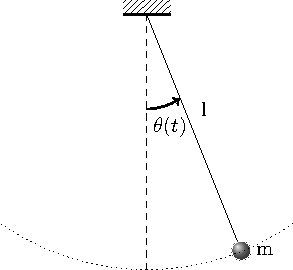
\includegraphics[width=0.4\linewidth]{imgs/pendule.pdf}}

\vspace{6mm}



Le pendule a l'équation du mouvement :

\begin{align}
\ddot{\theta} &= - \frac{g}{l} sin(\theta)
\end{align}
Pour les petites amplitudes d'oscillation, $\theta \ll 1$, on peut faire l'approximation $sin(\theta) \approx \theta$, on retrouve alors l’équation différentielle d’un oscillateur harmonique:

\begin{align}
\label{eq:eqdiff}
\ddot{\theta} &= - \frac{g}{l} \theta
\end{align}

La solution exacte de cette équation est simplement:
\begin{align}
\label{eq:solexacte}
\theta (t) &= \theta_0 \ cos(\omega_0 t)
\end{align}
où $\omega_0 = \sqrt{g/l}$ et nous avons supposé que le pendule partait du repos avec un déplacement initial $\theta_0 =0.2 \ rad$.


Nous allons transformer l'équation différentielle d’ordre 2 (Eq. (\ref{eq:eqdiff})) en deux équations différentielles d’ordre 1 afin de pouvoir utiliser simplement la méthode d’Euler. En posant $\omega (t)= \dot{\theta}(t)$ la vitesse angulaire du pendule, on obtient le système de deux fonctions inconnues suivant :
\begin{align}
\dot{\theta} (t) &= \omega (t) \\
\dot{\omega }(t) &= - \omega_0^2 \ \theta (t)
\end{align}
Pour résoudre ce système nous devons connaître les deux conditions initiales suivantes :
\begin{align*}
\theta(0) &= \theta_0 \\
\omega (0) &= 0
\end{align*}


\subex{a)}
Définir une fonction \Verb!sol_exacte(t)! qui renvoie la solution exacte de l'oscillateur harmonique donnée par l'équation (\ref{eq:solexacte}). Tracer cette solution pour $t \in [0,10]$ et pour un pas de $\Delta t = 0.01$ s.

% --- begin hint in exercise ---

\paragraph{Indication.}
\begin{itemize}
\item Utiliser la fonction \texttt{numpy.arange()} pour créer le vecteur temps \texttt{t}.

\item Utiliser la fonction \texttt{matplotlib.pyplot.plot()} pour tracer \Verb!sol_exacte(t)!.
\end{itemize}

\noindent
% --- end hint in exercise ---


% --- begin solution of exercise ---
\paragraph{Solution.}
Le programme Python qui renvoie et trace la solution exacte de l'oscillateur harmonique est le suivant:

\begin{cod}{cbg_gray}\begin{minted}[fontsize=\fontsize{9pt}{9pt},linenos=false,mathescape,baselinestretch=1.0,fontfamily=tt,xleftmargin=2mm]{python}
import numpy as np
import matplotlib.pyplot as plt
# SYSTÈME: PENDULE SIMPLE
g = 9.8 # accélération de pesanteur [m/s^2]
l = 1 # longeur du pendule [m]
dt = 0.01 # pas du temps [s]
Tf = 10 # temps finale de la simulation [s]
theta0 = 0.2 # angle initiale [rad]
omega0 = np.sqrt(g/l) 
# SOLUTION EXACTE
def pendule_exacte(t):
    return theta0 * np.cos(omega0 * t)
t = np.arange(0, Tf, dt)

plt.plot(t, pendule_exacte(t), linewidth=2, label="sol exacte")
plt.legend()
plt.ylabel("Amplitude d'oscillation [rad]")
plt.xlabel("Temps [s]")
plt.title("Oscillateur Harmonique")
plt.show()
\end{minted}
\end{cod}
\noindent

L'exécution de ce programme donne la figure suivante:



\vspace{6mm}

% inline figure
\centerline{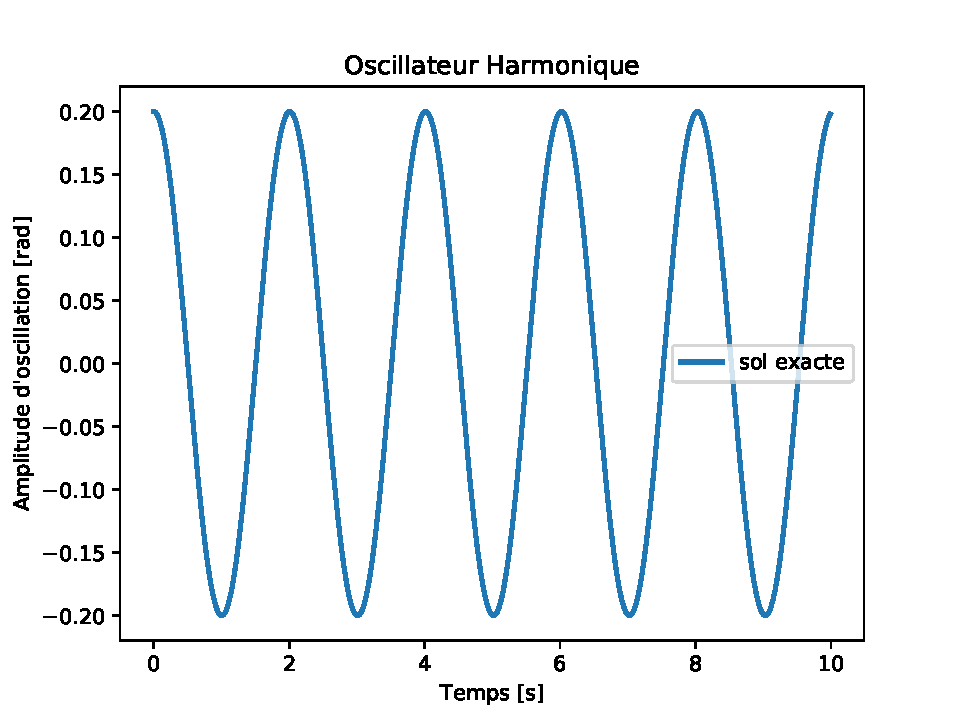
\includegraphics[width=0.7\linewidth]{scripts/sol_exacte.pdf}}

\vspace{6mm}



% --- end solution of exercise ---

\subex{b)}
Rappeler l'expression de la méthode \emph{d'Euler explicite} pour ce système.


% --- begin solution of exercise ---
\paragraph{Solution.}
\begin{align}
\label{eq:euler_exp}
\pmb{u}_{k+1}  &= \pmb{u}_k + \Delta t \pmb{A} \cdot \pmb{u}_k = (\pmb{I} + \Delta t  \pmb{A}) \cdot \pmb{u}_k
\end{align}

Où $\pmb{u}_k= \left(\begin{array}{c} \theta_k \\ \omega_k \end{array}\right)$, $\pmb{A}= \left(\begin{array}{ll} 0&1 \\ - g/l& 0 \end{array}\right)$ et $\pmb{I}$ est la matrice identité.

% --- end solution of exercise ---

\subex{c)}
Calculer $\pmb{u}= \left(\begin{array}{c} \theta (t) \\ \omega (t) \end{array}\right)$ avec la méthode d'Euler explicite pour $t \in [0, 10]$ et pour un pas d’intégration $\Delta t = 0.01$ s.

Tracer:
\begin{itemize}
\item Dans un même graphique, la variation de l'amplitude d'oscillation $\theta$ en fonction du temps $t$ et le diagramme des phases (vitesse angulaire $\omega$ en fonction de $\theta$).

\item Dans un graphique 3D, la vitesse angulaire $\omega$ et l'amplitude d'oscillation $\theta$ en fonction du temps $t$.
\end{itemize}

\noindent
Que remarquez-vous pour le résultat trouvé?

% --- begin hint in exercise ---

\paragraph{Indication.}
On vous donne les instructions nécessaires pour reproduire un graphique en 3D:
\begin{cod}{cbg_gray}\begin{minted}[fontsize=\fontsize{9pt}{9pt},linenos=false,mathescape,baselinestretch=1.0,fontfamily=tt,xleftmargin=2mm]{python}
from mpl_toolkits.mplot3d.axes3d import Axes3D
plt.figure()
ax = plt.axes(projection="3d")
ax.plot(....)
\end{minted}
\end{cod}
\noindent

% --- end hint in exercise ---


% --- begin solution of exercise ---
\paragraph{Solution.}
\begin{cod}{cbg_gray}\begin{minted}[fontsize=\fontsize{9pt}{9pt},linenos=false,mathescape,baselinestretch=1.0,fontfamily=tt,xleftmargin=2mm]{python}
#%% EULER EXPLICITE
A = np.array([[0, 1], [- omega0**2, 0]])
nsteps = int(Tf/dt)
# CONDITIONS INITIALES: à t = 0; theta = theta0, omega = 0
u0 = np.array([theta0, 0])

Texp = np.zeros(nsteps)
Uexp = np.zeros((2, nsteps))
Texp[0] = 0.0
Uexp[:,0] = u0
# ITÉRATION
for k in range(nsteps-1):
    Texp[k+1] = Texp[k] + dt
    Uexp[:,k+1] = np.dot((np.eye(2) + dt * A), Uexp[:,k])
    
plt.figure(figsize=(10,5))
# PLOT POSITION vs TEMPS
plt.subplot(1,2,1)
plt.plot(Texp,Uexp[0,:], linewidth=2)
plt.xlabel("Temps [s]")
plt.ylabel("Amplitude d'oscillation [rad]")
plt.title("Oscillateur Harmonique (Euler explicite)")
# DIAGRAMME DE PHASE 2D
plt.subplot(1,2,2)
plt.plot(Uexp[0,:],Uexp[1,:], linewidth=2)
plt.xlabel("Amplitude d'oscillation [rad]")
plt.ylabel("Vitesse angulaire [rad/s]")
plt.title("Espace des phases (Euler explicite)")
plt.savefig("Pendule_EulerExp1D.png"); plt.savefig("Pendule_EulerExp1D.pdf")
# DIAGRAMME DE PHASE 3D
from mpl_toolkits.mplot3d.axes3d import Axes3D
plt.figure()
ax = plt.axes(projection="3d")
ax.plot(Texp, Uexp[0,:],Uexp[1,:], linewidth=2)
ax.set_xlabel("Temps [s]")
ax.set_ylabel("Amplitude d'oscillation [rad]")
ax.set_zlabel("Vitesse angulaire [rad/s]")
ax.set_title("Espace des phases (Euler explicite)")
plt.show()
\end{minted}
\end{cod}
\noindent

L'exécution de ce programme donne les figures suivantes:



\vspace{6mm}

% inline figure
\centerline{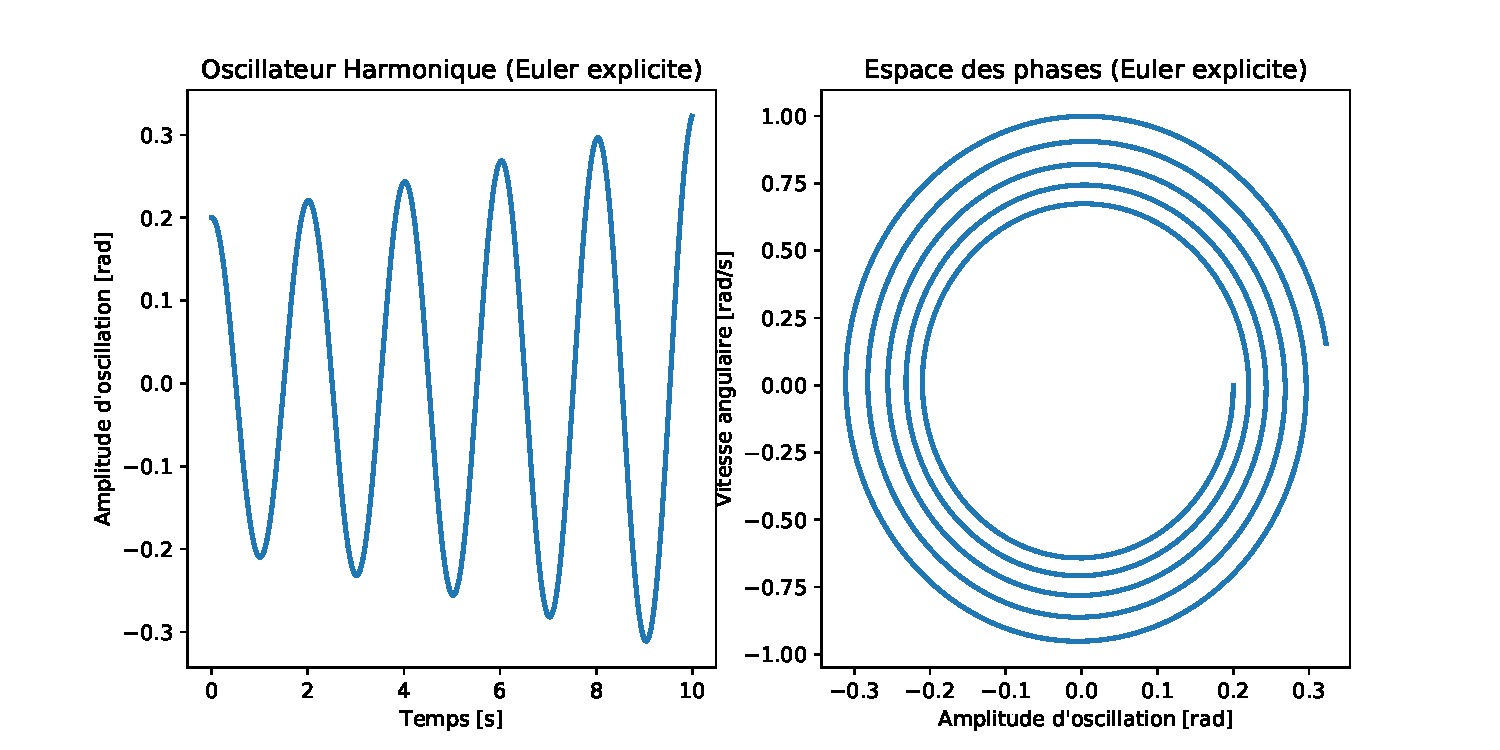
\includegraphics[width=1.0\linewidth]{scripts/Pendule_EulerExp1D.pdf}}

\vspace{6mm}



et la figure en 3D:



\vspace{6mm}

% inline figure
\centerline{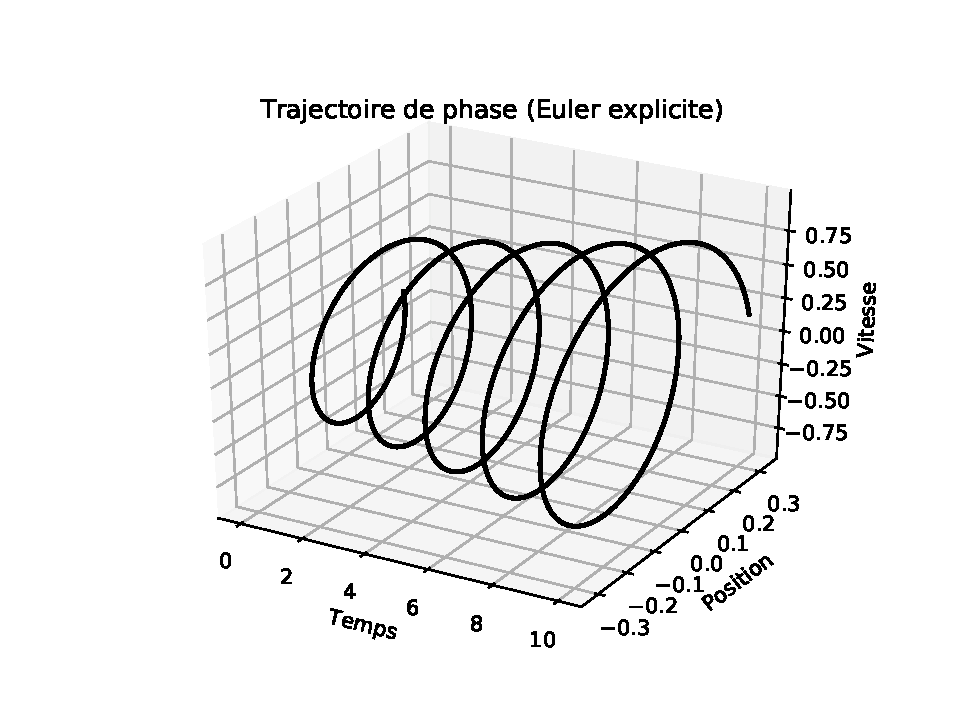
\includegraphics[width=1.0\linewidth]{scripts/Pendule_EulerExp3D.pdf}}

\vspace{6mm}




\begin{block_grayiconadmon}[Remarque]
Dans le cas d'intégration avec la méthode d'Euler explicite nous avons un problème d’augmentation d’amplitude dans le cas d’un oscillateur libre non amorti. Plus le temps de simulation est long, plus l'amplitude augmente, ce qui n'est pas ce que nous attendons de l'évolution du système dans le temps.
\end{block_grayiconadmon} % title: Remarque



% --- end solution of exercise ---

\subex{d)}
Rappeler l'expression de la méthode \emph{d'Euler implicite} pour ce système.


% --- begin solution of exercise ---
\paragraph{Solution.}
\begin{align}
\label{eq:euler_imp}
\pmb{u}_{k+1}  &=(\pmb{I} - \Delta t  \pmb{A})^{-1}  \cdot \pmb{u}_k
\end{align}

Où $\pmb{u}_k= \left(\begin{array}{c} \theta_k \\ \omega_k \end{array}\right)$, $\pmb{A}= \left(\begin{array}{ll} 0&1 \\ - g/l& 0 \end{array}\right)$ et $\pmb{I}$ est la matrice identité.

% --- end solution of exercise ---

\subex{e)}
Calculer $\pmb{u}= \left(\begin{array}{c} \theta (t) \\ \omega (t) \end{array}\right)$ avec la méthode d'Euler implicite pour $t \in [0, 10]$ et pour un pas d'integration $\Delta t = 0.01$ s.

Tracer:
\begin{itemize}
\item Dans un même graphique, la variation de l'amplitude d'oscillation $\theta$ en fonction du temps $t$ et le diagramme des phases (vitesse angulaire $\omega$ en fonction de $\theta$).

\item Dans un graphique 3D, la vitesse angulaire $\omega$ et l'amplitude d'oscillation $\theta$ en fonction du temps $t$.
\end{itemize}

\noindent
Que remarquez-vous pour le résultat trouvé?


% --- begin solution of exercise ---
\paragraph{Solution.}
\begin{cod}{cbg_gray}\begin{minted}[fontsize=\fontsize{9pt}{9pt},linenos=false,mathescape,baselinestretch=1.0,fontfamily=tt,xleftmargin=2mm]{python}
#%% EULER IMPLICITE
from numpy.linalg import inv
Timp = np.zeros(nsteps)
Uimp = np.zeros((2, nsteps))
Timp[0] = 0.0
Uimp[:,0] = u0
# ITÉRATION
for k in range(nsteps-1):
    Timp[k+1] = Timp[k] + dt
    Uimp[:,k+1] = np.dot(inv(np.eye(2) - dt * A), Uimp[:,k])
    
plt.figure(figsize=(10,5))
# PLOT POSITION vs TEMPS
plt.subplot(1,2,1)
plt.plot(Timp,Uimp[0,:], linewidth=2)
plt.xlabel("Temps [s]")
plt.ylabel("Amplitude d'oscillation [rad]")
plt.title("Oscillateur Harmonique (Euler implicite)")
# DIAGRAMME DE PHASE
plt.subplot(1,2,2)
plt.plot(Uimp[0,:],Uimp[1,:], linewidth=2)
plt.xlabel("Amplitude d'oscillation [rad]")
plt.ylabel("Vitesse angulaire [rad/s]")
plt.title("Espace des phases (Euler implicite)")
plt.savefig("Pendule_Eulerimp1D.png"); plt.savefig("Pendule_Eulerimp1D.pdf")
plt.show()
# DIAGRAMME DE PHASE 3D
plt.figure()
ax = plt.axes(projection="3d")
ax.plot(Timp, Uimp[0,:],Uimp[1,:], linewidth=2)
ax.set_xlabel("Temps [s]")
ax.set_ylabel("Amplitude d'oscillation [rad]")
ax.set_zlabel("Vitesse angulaire [rad/s]")
ax.set_title("Espace des phases (Euler implicite)")
plt.savefig("Pendule_Eulerimp3D.png"); plt.savefig("Pendule_Eulerimp3D.pdf")
plt.show()
\end{minted}
\end{cod}
\noindent

L'exécution de ce programme donne les figures suivantes:



\vspace{6mm}

% inline figure
\centerline{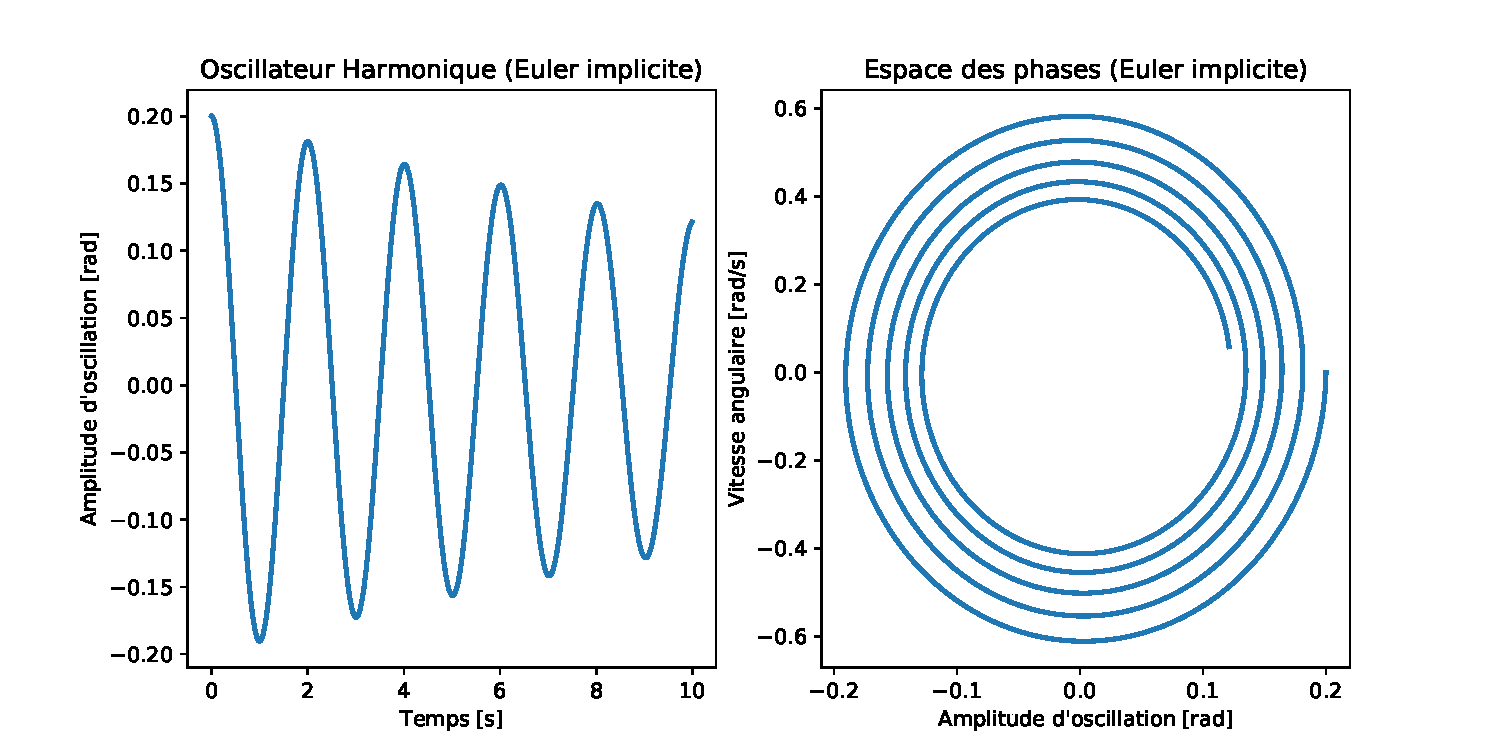
\includegraphics[width=1.0\linewidth]{scripts/Pendule_Eulerimp1D.pdf}}

\vspace{6mm}



et la figure en 3D:



\vspace{6mm}

% inline figure
\centerline{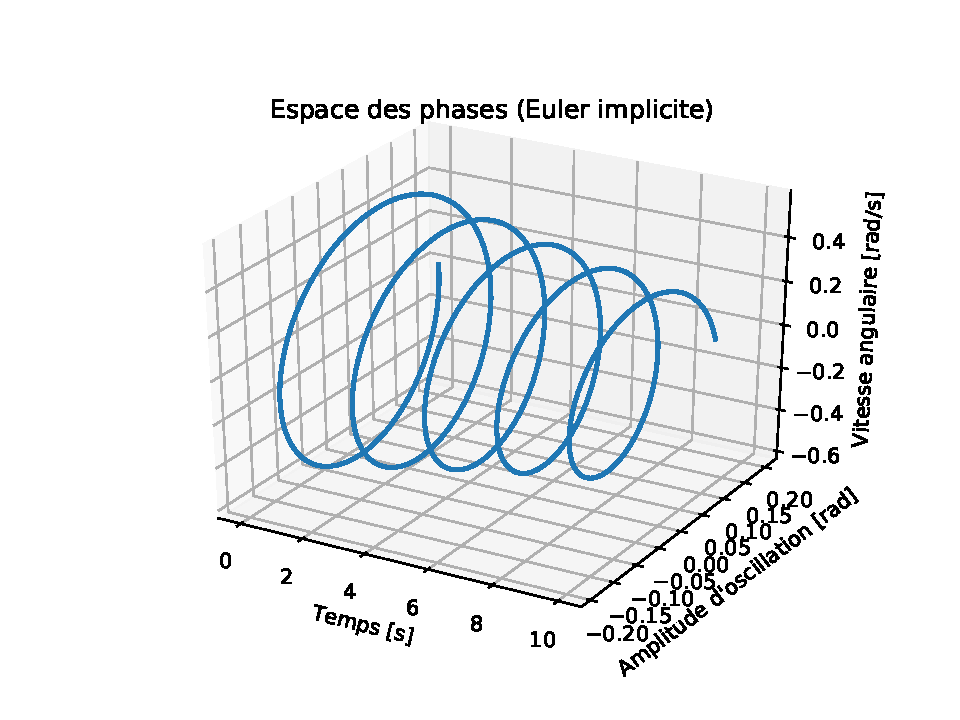
\includegraphics[width=1.0\linewidth]{scripts/Pendule_Eulerimp3D.pdf}}

\vspace{6mm}




\begin{block_grayiconadmon}[Remarque]
Dans le cas d'intégration avec la méthode d'Euler implicite nous avons un problème de diminution d’amplitude dans le cas d’un oscillateur libre non amorti. Plus le temps de simulation est long, plus l'amplitude diminue, ce qui n'est pas ce que nous attendons de l'évolution du système dans le temps.
\end{block_grayiconadmon} % title: Remarque



% --- end solution of exercise ---

\subex{f)}
Tracer dans un même graphique pour $t \in [0, 10]$ et avec un pas $\Delta t = 0.01$ s:
\begin{itemize}
\item \Verb!sol_exacte(t)! calculée dans \textbf{a)}.

\item $\theta (t)$ calculée dans \textbf{c)} par la méthode d'Euler explicite.

\item $\theta (t)$ calculée dans \textbf{e)} par la méthode d'Euler implicite.
\end{itemize}

\noindent
Que remarquez-vous si nous modifions la valeur du pas d’intégration par $\Delta~t =~0.001$~s? Expliquer le résultat trouvé.


% --- begin solution of exercise ---
\paragraph{Solution.}
\begin{cod}{cbg_gray}\begin{minted}[fontsize=\fontsize{9pt}{9pt},linenos=false,mathescape,baselinestretch=1.0,fontfamily=tt,xleftmargin=2mm]{python}
#%% ILLUSTRATION
plt.figure()
plt.plot(t, pendule_exacte(t), linewidth=2, label="sol exact")
plt.plot(t, Uexp[0,:], linewidth=2, linestyle='--', label="Euler explicite")
plt.plot(t, Uimp[0,:], linewidth=2, linestyle='--', label="Euler implicite")
plt.legend()
plt.xlabel("Temps [s]")
plt.ylabel("Amplitude d'oscillation [rad]")
plt.title("Oscillateur Harmonique avec "+ r"$\Delta t =$"+str(dt))
plt.savefig("Pendule_illustration.png"); plt.savefig("Pendule_illustration.pdf")
plt.show()
\end{minted}
\end{cod}
\noindent

Pour $\Delta t = 0.01$, l'exécution du code donne la figure suivante:



\vspace{6mm}

% inline figure
\centerline{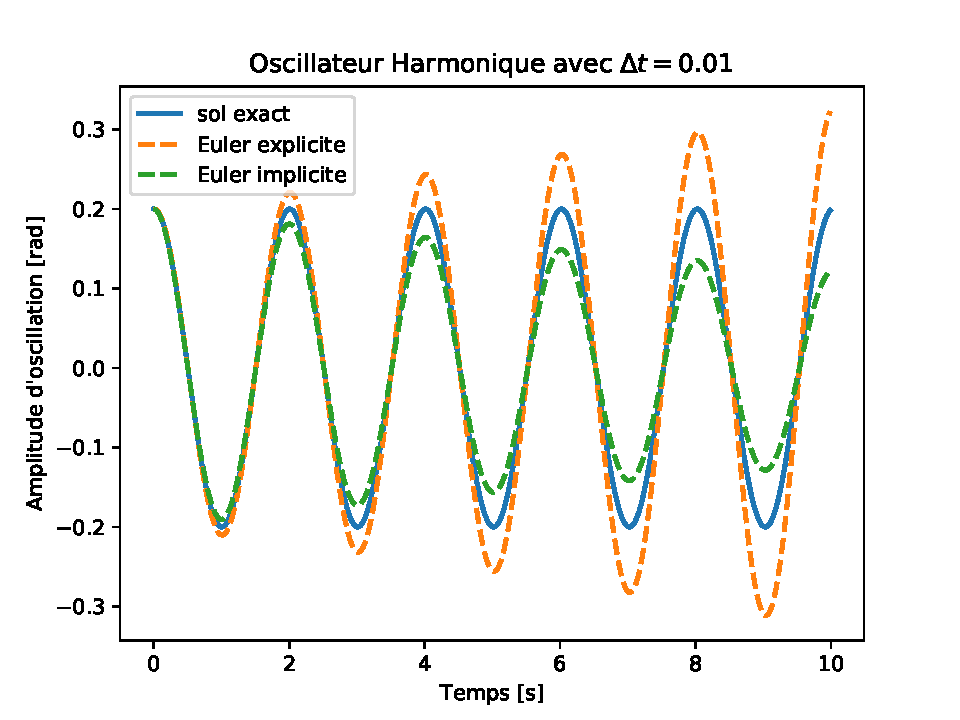
\includegraphics[width=0.7\linewidth]{scripts/Pendule_illustration.pdf}}

\vspace{6mm}



Pour $\Delta t = 0.001$, l'exécution du code donne la figure suivante:



\vspace{6mm}

% inline figure
\centerline{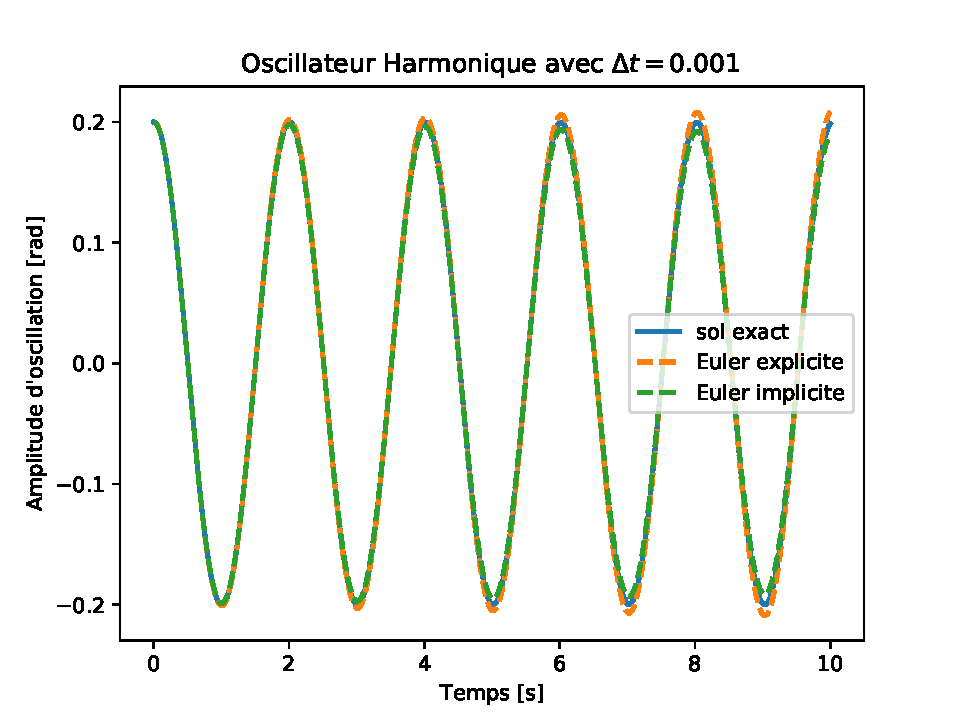
\includegraphics[width=0.7\linewidth]{scripts/Pendule_illustration1.pdf}}

\vspace{6mm}




\begin{block_grayiconadmon}[Remarque]
Les deux méthodes d'Euler, explicite et implicite, posent un problème fondamental avec ses amplitudes croissantes et décroissantes pour le cas d'oscillateur libre non amorti. Un très petit $\Delta t$ est nécessaire pour obtenir des résultats satisfaisants.

\emph{Plus la simulation est longue, plus $\Delta t$ doit être petit.}
\end{block_grayiconadmon} % title: Remarque



% --- end solution of exercise ---

\end{doconceexercise}
% --- end exercise ---




% --- begin exercise ---
\begin{doconceexercise}
\refstepcounter{doconceexercisecounter}

\exercisesection{Exercice \thedoconceexercisecounter: Comparaison des schémas d’Euler explicite et implicite}


On considère le problème de Cauchy:
\begin{align}
\frac{d z(t)}{dt} = 1 - \frac{t}{\mu}, \ t \in \Re, \ z(0) = z_0
\end{align}
On rappelle que la solution exacte de ce problème est donnée par:
\begin{align}
\label{eq:solexacte2}
z(t) = \mu -(\mu - z_0) e^{-\frac{t}{\mu}}
\end{align}

1. Définir une fonction \Verb!sol_exacte(t, mu, z0)! qui renvoie la solution exacte donnée par l'équation (\ref{eq:solexacte2}). Tracer sur un même graphique pour $\mu= 1$ et $z_0 \in \{0, 1, 2\}$ ces solutions. Soit $t \in [0,2]$ et pour un pas de $\Delta t = 0.1$ s.

2. Même questions pour $\mu= 0.05$ et $z_0 \in \{0, 1, 2\}$.

3. On suppose dans cette question que $\mu= 0.05$ et que $z_0  = 2$.


\subex{a)}
\begin{itemize}
\item Rappeler l'expression de la méthode \emph{d'Euler explicite} pour ce problème.

\item Calculer $z(t)$ avec la méthode \emph{d’Euler explicite} pour $t \in [0, 2]$ et pour un pas d’intégration $\Delta t = 0.1$ s.
\end{itemize}

\noindent
\subex{b)}
\begin{itemize}
\item Montrer que l'expression de la méthode \emph{d'Euler implicite} est:
\end{itemize}

\noindent
\begin{align*}
z_{n+1} = \frac{z_n + \Delta t}{1 + \frac{\Delta t}{\mu}}, \ n = 0, 1, 2, ..., N-1
\end{align*}
\begin{itemize}
\item Calculer $z(t)$ avec la méthode \emph{d’Euler implicite} pour $t \in [0, 2]$ et pour un pas d’intégration $\Delta t = 0.1$ s.
\end{itemize}

\noindent
\subex{c)}
Tracer dans un même graphique pour $t \in [0, 2]$ et avec des pas d'intégration
 $\Delta t = 0.5, 0.1, 0.05, 0.01, 0.005$ s:
\begin{itemize}
 \item La solution exacte: \Verb!sol_exacte(t, 0.05, 2)!

 \item $z(t)$ calculée par la méthode d'Euler explicite.

 \item $z(t)$ calculée par la méthode d'Euler explicite.
\end{itemize}

\noindent
 Que remarquez-vous pour les résultats trouvés? Quelle est la méthode la plus proche de la solution exacte?

\end{doconceexercise}
% --- end exercise ---


% !split


% --- begin exercise ---
\begin{doconceexercise}
\refstepcounter{doconceexercisecounter}

\exercisesection{Exercice \thedoconceexercisecounter: Atterrissage d'un vaisseau spatial}




\vspace{6mm}

% inline figure
\centerline{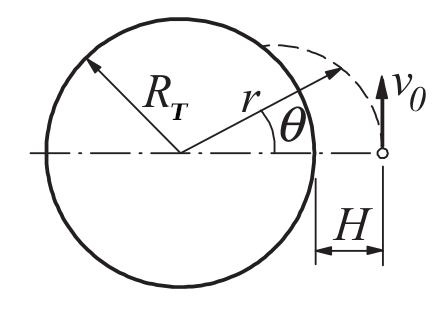
\includegraphics[width=0.4\linewidth]{imgs/spacecraft.png}}

\vspace{6mm}



Un vaisseau spatial est lancé à l'altitude $H = 772 \ km$ au-dessus du niveau de la mer avec la vitesse $v_0 = 6700 \ m/s$ dans la direction indiquée sur la figure ci-dessus. Les équations différentielles décrivant le mouvement du vaisseau spatial sont:
\begin{align*}
\ddot{r} &= r \dot{\theta}^2 - \frac{G M_T}{r^2} \\
\ddot{\theta} &= - \frac{2 \dot{r} \dot{\theta}}{r}
\end{align*}
où $r$ et $\theta$ sont les coordonnées polaires du vaisseau spatial. Les constantes impliquées dans le mouvement sont:
\begin{itemize}
\item $G = 6.672 \times 10^{−11} \ m^3 kg^{−1} s^{−2}$ = constante gravitationnelle universelle.

\item $M_T = 5.9742 \times 10^{24} \ kg$ = masse de la terre.

\item $R_T = 6378.14 \ km$ = rayon de la terre au niveau de la mer.
\end{itemize}

\noindent
\subex{a)}
Dériver les équations différentielles du premier ordre et les conditions initiales de la forme $\dot{y} = F (t, y)$, $y(0) = b$.

\subex{b)}
Utiliser la méthode Runge-Kutta du quatrième ordre (RK4) pour intégrer les équations depuis le lancement jusqu'à ce que le vaisseau spatial touche la terre. Déterminez $\theta$ au site d'impact.

\end{doconceexercise}
% --- end exercise ---


% ------------------- end of main content ---------------

% #ifdef PREAMBLE
\end{document}
% #endif

